\documentclass[12pt,a4paper]{article}
\usepackage[utf8]{inputenc}
\usepackage[T1]{fontenc}
\usepackage{amsmath}
\usepackage{amsfonts}
\usepackage{amssymb}
\usepackage{graphicx}
\usepackage{hyperref}
\usepackage[polish]{babel}
\usepackage{algorithm}
\usepackage{algpseudocode}
\usepackage{booktabs}
\usepackage{float}
\usepackage{subcaption}
\usepackage{changepage}
\usepackage{geometry}

% Marginesy
\geometry{a4paper, margin=2.5cm}

% Fix for Polish algorithm name
\makeatletter
\def\ALG@name{Algorytm}
\makeatother

% Allow algorithms to float but keep them in the same section
% \floatplacement{algorithm}{tbp} % Usunięto globalne ustawienie pływania dla algorytmów

% Make font smaller in algorithm listings
\makeatletter
\algrenewcommand\ALG@beginalgorithmic{\footnotesize}
\makeatother

\title{Sprawozdanie z implementacji algorytmów MSLS, ILS i LNS dla zmodyfikowanego problemu komiwojażera}
\author{Filip Rosiak 151799  \and Eryk Stec 152948}
\date{\today}

\begin{document}

\maketitle

\begin{abstract}
W niniejszym sprawozdaniu przedstawiono implementację i analizę trzech rozszerzeń algorytmu przeszukiwania lokalnego dla zmodyfikowanego problemu komiwojażera: Multiple Start Local Search (MSLS), Iterated Local Search (ILS) oraz Large Neighborhood Search (LNS). Jako bazowy algorytm lokalnego przeszukiwania wykorzystano najlepszy wariant z poprzedniego zadania, czyli Candidate Steepest z k=10. Opisano zastosowane mechanizmy perturbacji dla ILS (mała perturbacja przez losowe ruchy) i LNS (typu Destroy-Repair z heurystyczną naprawą). Porównano wyniki uzyskane przez zaimplementowane metaheurystyki, w tym wariant LNS bez lokalnego przeszukiwania po naprawie (LNSa). Eksperymenty przeprowadzono na instancjach kroa200 i krob200, zgodnie z warunkami opisanymi w zadaniu, w tym z wykorzystaniem średniego czasu MSLS jako limitu czasowego dla ILS i LNS.
\end{abstract}

\section{Opis problemu}
Rozważany problem jest modyfikacją klasycznego problemu komiwojażera. Dany jest zbiór wierzchołków i symetryczna macierz odległości pomiędzy dowolną parą wierzchołków. Zadanie polega na ułożeniu dwóch rozłącznych zamkniętych ścieżek (cykli), każda zawierająca 50\% wierzchołków (jeżeli liczba wierzchołków w instancji nie jest parzysta, to pierwsza ścieżka zawiera jeden wierzchołek więcej), minimalizując łączną długość obu ścieżek.

Do testów wykorzystano instancje \texttt{kroa200} i \texttt{krob200} z biblioteki TSPLib. Są to dwuwymiarowe instancje euklidesowe, gdzie dla każdego wierzchołka podane są dwie współrzędne, a odległość pomiędzy wierzchołkami jest odległością euklidesową zaokrąglaną do liczby całkowitej.

\section{Zaimplementowane algorytmy}
W ramach zadania zaimplementowano i porównano następujące metaheurystyki, oparte na najlepszym algorytmie lokalnego przeszukiwania (LS) z poprzedniego zadania - Candidate Steepest (k=10) z sąsiedztwem Edge Exchange i startem z losowych rozwiązań:

\subsection{Multiple Start Local Search (MSLS)}
Algorytm polega na wielokrotnym uruchomieniu bazowego algorytmu lokalnego przeszukiwania (LS) z różnych, losowo generowanych rozwiązań początkowych. Wynikiem końcowym jest najlepsze rozwiązanie znalezione spośród wszystkich uruchomień LS. W eksperymentach wykonano 200 iteracji (uruchomień LS) dla każdej instancji. Pseudokod przedstawiono w Algorytmie~\ref{alg:msls}.

\begin{algorithm}[H]
\caption{Algorytm: Multiple Start Local Search (MSLS)}
\label{alg:msls}
\begin{algorithmic}[1]
\Require \texttt{instance}, \texttt{base\_local\_search}, \texttt{iterations}
\Ensure \texttt{best\_overall\_solution}
\State \texttt{best\_overall\_solution} $\leftarrow$ \texttt{null}
\State \texttt{min\_cost} $\leftarrow$ $\infty$
\For{$i \leftarrow 1$ to \texttt{iterations}}
    \State \texttt{start\_solution} $\leftarrow$ \texttt{generate\_random\_solution(instance)}
    \State \texttt{current\_solution} $\leftarrow$ \texttt{base\_local\_search(start\_solution, instance)}
    \State \texttt{current\_cost} $\leftarrow$ \texttt{calculate\_cost(current\_solution, instance)}
    \If{\texttt{current\_cost < min\_cost}}
        \State \texttt{min\_cost} $\leftarrow$ \texttt{current\_cost}
        \State \texttt{best\_overall\_solution} $\leftarrow$ \texttt{current\_solution}
    \EndIf
\EndFor
\State \Return \texttt{best\_overall\_solution}
\end{algorithmic}
\end{algorithm}

\subsection{Iterated Local Search (ILS)}
Algorytm rozpoczyna od znalezienia lokalnego optimum za pomocą bazowego LS. Następnie iteracyjnie wykonuje kroki perturbacji i lokalnego przeszukiwania. Perturbacja polega na wprowadzeniu niewielkich, losowych zmian w bieżącym najlepszym rozwiązaniu, aby umożliwić ucieczkę z lokalnego optimum. Po perturbacji ponownie stosowany jest bazowy LS. Nowe rozwiązanie jest akceptowane, jeśli jest lepsze od dotychczas najlepszego. Jako perturbację zaimplementowano \textbf{Perturbację 1}, która wykonuje 10 losowych ruchów (wymiana wierzchołków lub krawędzi) bez sprawdzania ich wpływu na koszt. Warunkiem stopu dla ILS był limit czasowy równy średniemu czasowi wykonania MSLS dla danej instancji. Pseudokod przedstawiono w Algorytmie~\ref{alg:ils}.

\begin{algorithm}[H]
\caption{Algorytm: Iterated Local Search (ILS)}
\label{alg:ils}
\begin{algorithmic}[1]
\Require \texttt{instance}, \texttt{base\_local\_search}, \texttt{perturbation}, \texttt{time\_limit}
\Ensure \texttt{best\_solution}
\State \texttt{start\_solution} $\leftarrow$ \texttt{generate\_random\_solution(instance)}
\State \texttt{best\_solution} $\leftarrow$ \texttt{base\_local\_search(start\_solution, instance)}
\State \texttt{best\_cost} $\leftarrow$ \texttt{calculate\_cost(best\_solution, instance)}
\State \texttt{start\_time} $\leftarrow$ \texttt{current\_time()}
\While{\texttt{current\_time()} - \texttt{start\_time} < \texttt{time\_limit}}
    \State \texttt{current\_solution} $\leftarrow$ \texttt{clone(best\_solution)}
    \State \texttt{perturbation(current\_solution, instance)}
    \State \texttt{current\_solution} $\leftarrow$ \texttt{base\_local\_search(current\_solution, instance)}
    \State \texttt{current\_cost} $\leftarrow$ \texttt{calculate\_cost(current\_solution, instance)}
    \If{\texttt{current\_cost < best\_cost}}
        \State \texttt{best\_solution} $\leftarrow$ \texttt{current\_solution}
        \State \texttt{best\_cost} $\leftarrow$ \texttt{current\_cost}
    \EndIf
\EndWhile
\State \Return \texttt{best\_solution}
\end{algorithmic}
\end{algorithm}

\subsection{Large Neighborhood Search (LNS)}
Podobnie jak ILS, algorytm LNS iteracyjnie modyfikuje rozwiązanie, ale wykorzystuje bardziej radykalną perturbację typu Destroy-Repair. Krok \textbf{Destroy} polega na usunięciu pewnego odsetka (w implementacji 20\%) losowo wybranych wierzchołków z bieżącego rozwiązania. Krok \textbf{Repair} polega na ponownym wstawieniu usuniętych wierzchołków do częściowego rozwiązania za pomocą heurystyki konstrukcyjnej - w tym przypadku zaimplementowano wariant heurystyki \textbf{Ważony 2-żal} (Weighted Regret) do naprawy rozwiązania. Perturbację tę nazwano \textbf{Perturbacja Destroy-Repair (20\%)}. Po naprawie (opcjonalnie) stosowany jest bazowy LS. Zaimplementowano dwie wersje:
\begin{itemize}
    \item \textbf{LNS}: Zastosowanie bazowego LS po kroku Repair.
    \item \textbf{LNSa}: Bez stosowania bazowego LS po kroku Repair (LS stosowane tylko na początku, o ile start był losowy).
\end{itemize}
Warunkiem stopu dla LNS/LNSa był limit czasowy równy średniemu czasowi wykonania MSLS dla danej instancji. Pseudokod przedstawiono w Algorytmie~\ref{alg:lns}.

\begin{algorithm}[H]
\caption{Algorytm: Large Neighborhood Search (LNS)}
\label{alg:lns}
\begin{algorithmic}[1]
\Require \texttt{instance}, \texttt{base\_local\_search}, \texttt{destroy}, \texttt{repair}, \texttt{apply\_ls\_after\_repair}, \texttt{apply\_ls\_to\_initial}, \texttt{time\_limit}
\Ensure \texttt{best\_solution}
\State \texttt{best\_solution} $\leftarrow$ \texttt{generate\_random\_solution(instance)}
\If{\texttt{apply\_ls\_to\_initial}}
    \State \texttt{best\_solution} $\leftarrow$ \texttt{base\_local\_search(best\_solution, instance)}
\EndIf
\State \texttt{best\_cost} $\leftarrow$ \texttt{calculate\_cost(best\_solution, instance)}
\State \texttt{start\_time} $\leftarrow$ \texttt{current\_time()}
\While{\texttt{current\_time()} - \texttt{start\_time} < \texttt{time\_limit}}
    \State \texttt{current\_solution} $\leftarrow$ \texttt{clone(best\_solution)}
    \State \texttt{destroyed\_nodes} $\leftarrow$ \texttt{destroy(current\_solution, instance)}
    \State \texttt{repair(current\_solution, destroyed\_nodes, instance)} \Comment{Używa Weighted Regret}
    \If{\texttt{apply\_ls\_after\_repair}}
        \State \texttt{current\_solution} $\leftarrow$ \texttt{base\_local\_search(current\_solution, instance)}
    \EndIf
    \State \texttt{current\_cost} $\leftarrow$ \texttt{calculate\_cost(current\_solution, instance)}
    \If{\texttt{current\_cost < best\_cost}}
        \State \texttt{best\_solution} $\leftarrow$ \texttt{current\_solution}
        \State \texttt{best\_cost} $\leftarrow$ \texttt{current\_cost}
    \EndIf
\EndWhile
\State \Return \texttt{best\_solution}
\end{algorithmic}
\end{algorithm}

\section{Wyniki eksperymentów}
Każdy z algorytmów (MSLS, ILS, LNS, LNSa) został uruchomiony 10 razy dla każdej instancji (kroa200, krob200). MSLS wykonywał 200 iteracji bazowego LS (Candidate Steepest k=10). Algorytmy ILS, LNS i LNSa działały przez czas równy średniemu czasowi wykonania MSLS dla danej instancji. Poniżej przedstawiono zagregowane wyniki.

\begin{table}[H]
\centering
\caption{Wyniki algorytmów (średnia, zakres [min - max] kosztu, średni czas, średnia liczba iteracji dla ILS/LNS)}
\label{tab:results}
\resizebox{\textwidth}{!}{%
\begin{tabular}{@{}lccccc@{}}
\toprule
\textbf{Algorytm} & \textbf{Koszt min} & \textbf{Koszt śr.} & \textbf{Koszt max} & \textbf{Czas śr. [ms]} & \textbf{Iteracje śr.} \\
\midrule
\multicolumn{6}{c}{\textbf{Instancja kroa200}} \\
\midrule
MSLS (200 iter.)        & 35608 & 36599.90 & 37296 & 9332.70 & N/A \\
ILS (Perturbacja 1, 10 ruchów)   & 35795 & 36500.70 & 37219 & 9365.10 & 174.8 \\
LNS (Destroy-Repair 20\%)  & 36233 & 36771.90 & 37456 & 9358.00 & 165.3 \\
LNSa (Destroy-Repair 20\%) & \textbf{30832} & \textbf{32111.00} & \textbf{33452} & 9334.90 & 1922.8 \\
\midrule
\multicolumn{6}{c}{\textbf{Instancja krob200}} \\
\midrule
MSLS (200 iter.)        & 36237 & 36957.30 & 37474 & 5679.10 & N/A \\
ILS (Perturbacja 1, 10 ruchów)   & 36351 & 36947.00 & 37580 & 5692.30 & 192.7 \\
LNS (Destroy-Repair 20\%)  & 36506 & 37082.00 & 37678 & 5695.70 & 176.2 \\
LNSa (Destroy-Repair 20\%) & \textbf{31598} & \textbf{32315.50} & \textbf{32825} & 5680.10 & 1902.4 \\
\bottomrule
\end{tabular}%
}
\end{table}

\section{Wizualizacje}
Poniżej przedstawiono wizualizacje najlepszych rozwiązań znalezionych przez poszczególne algorytmy dla obu instancji.

\begin{figure}[H]
\begin{adjustwidth}{-1cm}{-1cm} % Dostosuj marginesy dla tej figury
    \centering
    \begin{subfigure}[b]{0.5\textwidth}
        \centering
        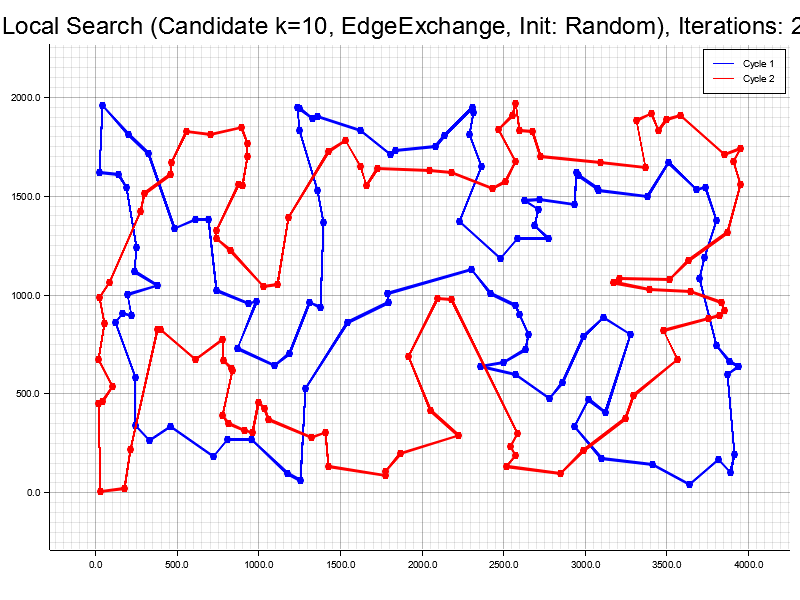
\includegraphics[width=\textwidth]{figures/kroa200_MSLS_Base_Local_Search_Candidate_k_10_EdgeExchange_Init_Random__Iterations_200_.png}
        \caption{kroa200}
    \end{subfigure}%
    \hfill
    \begin{subfigure}[b]{0.5\textwidth}
        \centering
        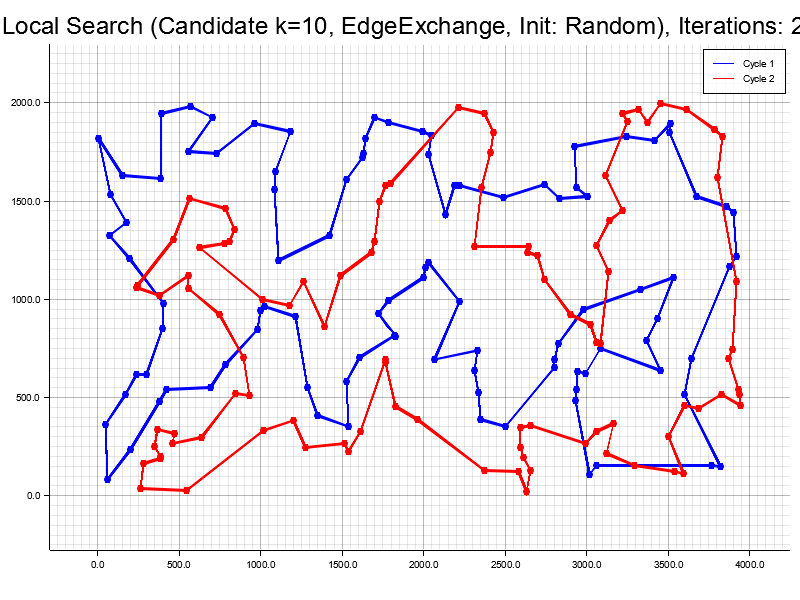
\includegraphics[width=\textwidth]{figures/krob200_MSLS_Base_Local_Search_Candidate_k_10_EdgeExchange_Init_Random__Iterations_200_.png}
        \caption{krob200}
    \end{subfigure}
    \caption{Wizualizacje najlepszych rozwiązań dla MSLS}
    \label{fig:msls}
\end{adjustwidth}
\end{figure}

\begin{figure}[H]
\begin{adjustwidth}{-1cm}{-1cm}
    \centering
    \begin{subfigure}[b]{0.5\textwidth}
        \centering
        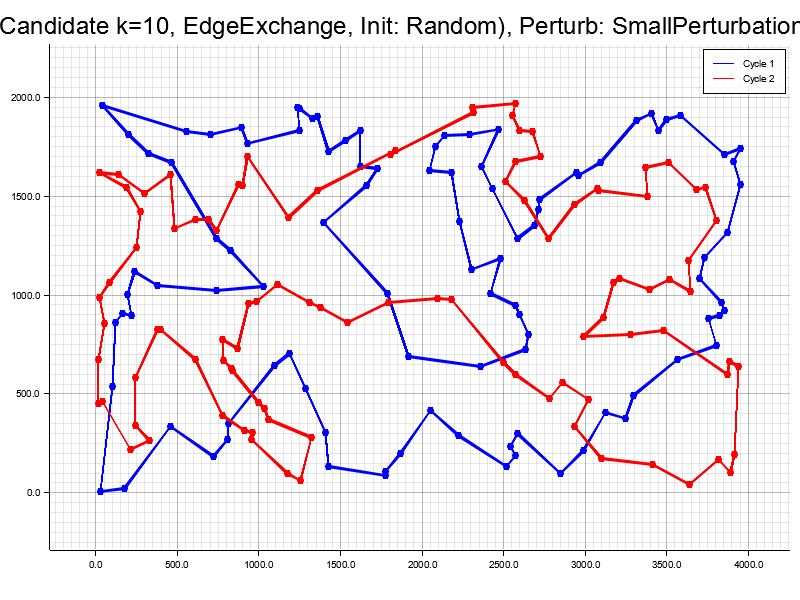
\includegraphics[width=\textwidth]{figures/kroa200_ILS_Base_Local_Search_Candidate_k_10_EdgeExchange_Init_Random__Perturb_SmallPerturbation_n_moves_10_.png}
        \caption{kroa200}
    \end{subfigure}%
    \hfill
    \begin{subfigure}[b]{0.5\textwidth}
        \centering
        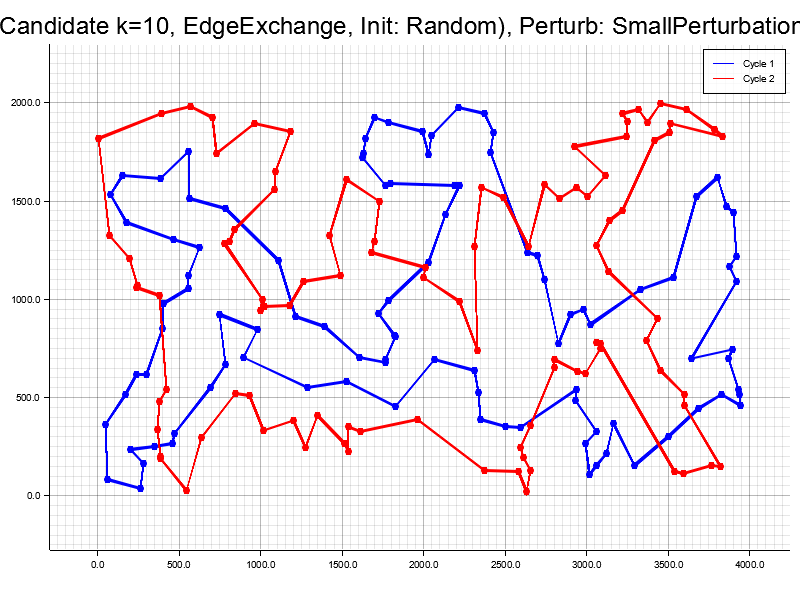
\includegraphics[width=\textwidth]{figures/krob200_ILS_Base_Local_Search_Candidate_k_10_EdgeExchange_Init_Random__Perturb_SmallPerturbation_n_moves_10_.png}
        \caption{krob200}
    \end{subfigure}
    \caption{Wizualizacje najlepszych rozwiązań dla ILS (Perturbacja 1, 10 losowych ruchów)}
    \label{fig:ils}
\end{adjustwidth}
\end{figure}

\begin{figure}[H]
\begin{adjustwidth}{-1cm}{-1cm}
    \centering
    \begin{subfigure}[b]{0.5\textwidth}
        \centering
        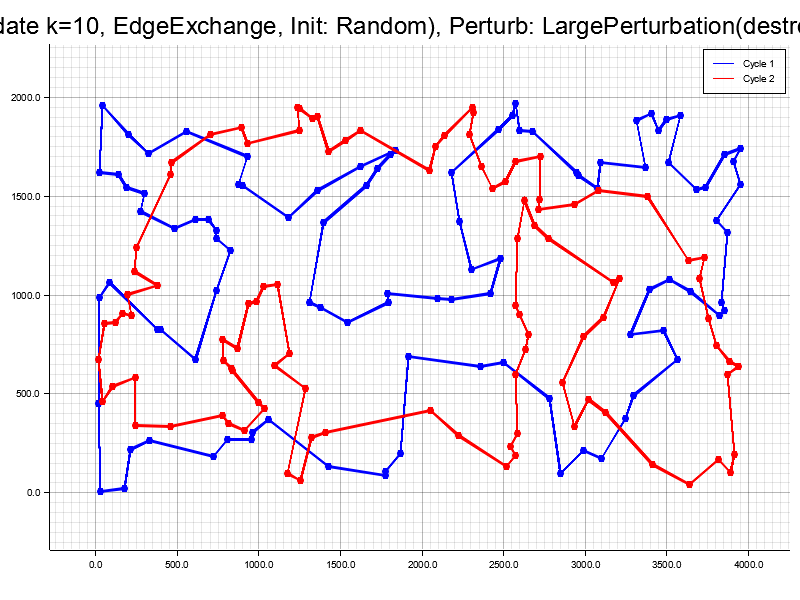
\includegraphics[width=\textwidth]{figures/kroa200_LNS_Base_Local_Search_Candidate_k_10_EdgeExchange_Init_Random__Perturb_LargePerturbation_destroy_0_20__LS_on_Initial_.png}
        \caption{kroa200}
    \end{subfigure}%
    \hfill
    \begin{subfigure}[b]{0.5\textwidth}
        \centering
        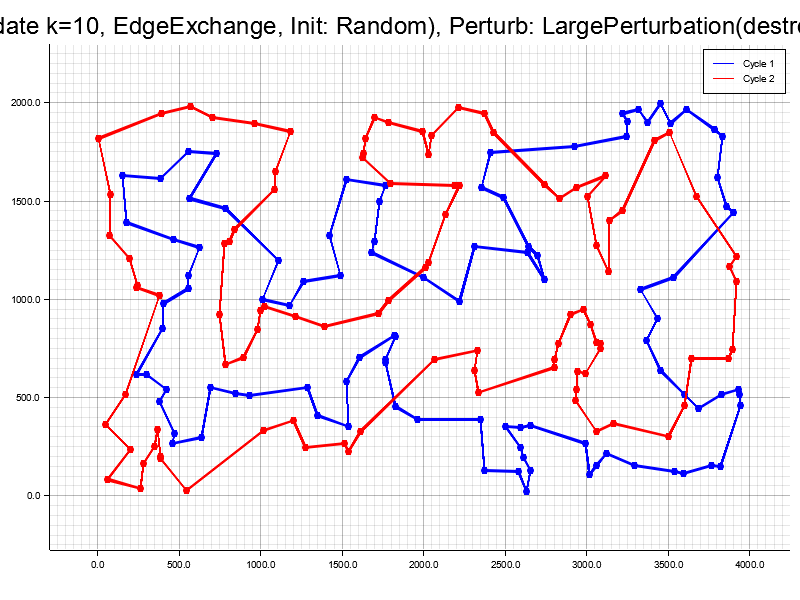
\includegraphics[width=\textwidth]{figures/krob200_LNS_Base_Local_Search_Candidate_k_10_EdgeExchange_Init_Random__Perturb_LargePerturbation_destroy_0_20__LS_on_Initial_.png}
        \caption{krob200}
    \end{subfigure}
    \caption{Wizualizacje najlepszych rozwiązań dla LNS (Destroy-Repair 20\%)}
    \label{fig:lns}
\end{adjustwidth}
\end{figure}

\begin{figure}[H]
\begin{adjustwidth}{-1cm}{-1cm}
    \centering
    \begin{subfigure}[b]{0.5\textwidth}
        \centering
        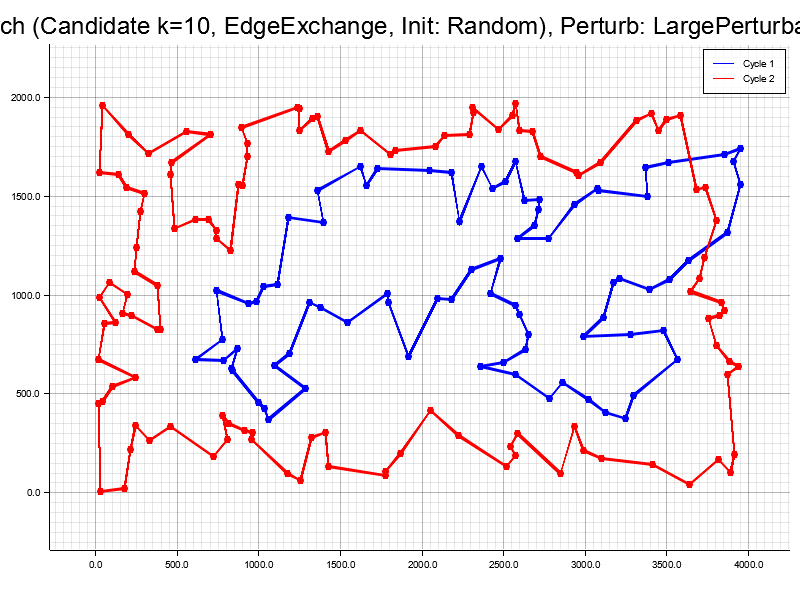
\includegraphics[width=\textwidth]{figures/kroa200_LNSa_no_LS_after_repair__Base_Local_Search_Candidate_k_10_EdgeExchange_Init_Random__Perturb_LargePerturbation_destroy_0_20__LS_on_Initial_.png}
        \caption{kroa200}
    \end{subfigure}%
    \hfill
    \begin{subfigure}[b]{0.5\textwidth}
        \centering
        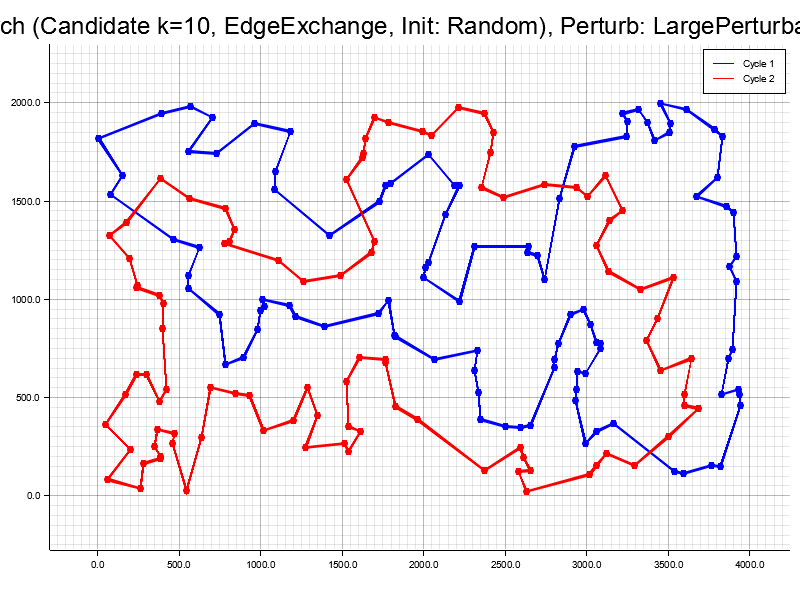
\includegraphics[width=\textwidth]{figures/krob200_LNSa_no_LS_after_repair__Base_Local_Search_Candidate_k_10_EdgeExchange_Init_Random__Perturb_LargePerturbation_destroy_0_20__LS_on_Initial_.png}
        \caption{krob200}
    \end{subfigure}
    \caption{Wizualizacje najlepszych rozwiązań dla LNSa (Destroy-Repair 20\%, bez LS po naprawie)}
    \label{fig:lnsa}
\end{adjustwidth}
\end{figure}

\section{Wnioski}
Na podstawie przeprowadzonych eksperymentów można wyciągnąć następujące wnioski dotyczące zaimplementowanych algorytmów MSLS, ILS i LNS dla rozważanego problemu:

\begin{enumerate}
    \item \textbf{Porównanie ILS/LNS z MSLS:} Zgodnie z wymaganiami zadania, dążono do tego, aby ILS i LNS dawały wyniki lepsze niż MSLS. Standardowe warianty ILS (z małą perturbacją) i LNS (z dużą perturbacją i LS po naprawie) uzyskały wyniki jakościowe (średni koszt) bardzo zbliżone, a nawet nieznacznie gorsze od MSLS w tym samym limicie czasowym (średni czas MSLS). LNS znalazł jednak najlepsze rozwiązanie minimalne dla instancji krob200.

    \item \textbf{Skuteczność LNSa:} Wariant LNS bez lokalnego przeszukiwania po fazie naprawy (LNSa) okazał się zdecydowanie najskuteczniejszy pod względem jakości znalezionych rozwiązań. Zarówno średni, jak i minimalny koszt uzyskany przez LNSa jest wyraźnie niższy niż dla pozostałych algorytmów. Jest to prawdopodobnie spowodowane możliwością wykonania znacznie większej liczby iteracji Destroy-Repair w tym samym limicie czasowym (średnio $\sim$1800-2000 iteracji LNSa vs $\sim$180-200 iteracji ILS/LNS), co pozwala na eksplorację większego obszaru przestrzeni rozwiązań. Pominięcie kosztownego kroku LS po każdej naprawie pozwala na częstsze stosowanie mechanizmu Destroy-Repair.

    \item \textbf{Liczba iteracji:} Jak wspomniano, liczba iteracji (perturbacji) wykonanych przez ILS i standardowy LNS w zadanym limicie czasowym jest stosunkowo niewielka (ok. 180-200), co wynika z faktu, że większość czasu zajmuje wykonanie bazowego algorytmu lokalnego przeszukiwania po każdej perturbacji. LNSa, pomijając ten krok, wykonuje około 10 razy więcej iteracji Destroy-Repair.

    \item \textbf{Rodzaj perturbacji:} Mała perturbacja w ILS (10 losowych ruchów) wydaje się być niewystarczająca, aby efektywnie uciec z lokalnych optimów i znaleźć znacząco lepsze rozwiązania niż MSLS w danym czasie. Duża perturbacja w LNS (Destroy 20\% + Repair Ważonym 2-żalem) w połączeniu z pominięciem LS po naprawie (LNSa) okazała się bardzo efektywną strategią dla tego problemu.

    \item \textbf{Kompromis jakość/czas:} Wszystkie algorytmy ILS i LNS działały w podobnym czasie (zgodnie z założeniem eksperymentu). Kluczową różnicą jest jakość. LNSa oferuje najlepszą jakość kosztem rezygnacji z intensyfikacji przez LS po każdej naprawie, co jednak okazuje się korzystne dzięki znacznie większej liczbie cykli Destroy-Repair. Standardowe ILS i LNS oferują jakość porównywalną z MSLS.

\end{enumerate}

Podsumowując, najskuteczniejszą zaimplementowaną strategią okazał się algorytm LNSa, który dzięki mechanizmowi Destroy-Repair z heurystyką Ważony 2-żal i rezygnacji z kosztownego kroku LS po naprawie, był w stanie znacząco poprawić jakość rozwiązania w porównaniu do MSLS, ILS i standardowego LNS w tym samym limicie czasowym.

\section{Kod źródłowy}
Pełny kod źródłowy implementacji wszystkich algorytmów jest dostępny w repozytorium GitHub:
\url{https://github.com/Veanir/imo-4}

\end{document} 